\chapter{Introduction}
For wildlife monitoring, typically camera traps are used. During daylight, normal cameras succeed in capturing detailed images.
But in the absence of daylight \textit{near-infrared} (NIR) cameras or normal cameras using incandescent lighting are necessary.
Near infrared light has a wavelength of between $750$ nm and $1400$ nm which lies outside the visible spectrum ($380$nm - $780$nm) \parencite{ISO.20473:2007}. 
Because of that, NIR cameras offer a significant advantage over conventional cameras using incandescent lighting.
Incandescent light flashes are visible to animals and may frighten them, which leads animals to avoid the camera location afterward.
Near-infrared light, however, is not visible to most animals, and thus cannot scare them.
However, unlike colored RGB images, NIR images lack colorization, which is essential for human comprehension and interpretation of visual information.
Also, some classification- and animal detection solutions may benefit from three-channel RGB images \parencite{cyclegan-camera-traps}.
Therefore, the conversion of NIR images to colored RGB images can combine the advantages of both methods:
Detail-rich images without scaring animals, that humans can easily interpret and classification and animal detection systems can benefit from.

Although colorizing NIR images is closely related to colorizing grayscale images (\textit{image colorization}), it differs in one important property:
The luminance of grayscale images captured in the visible spectrum is the same as the luminance of colored images, thus only chrominance must be estimated by image colorization systems.
However, the objects' reflection properties of near-infrared light differ from those of light from the visual spectrum.
Consequently, due to the differing luminance between RGB and NIR images, conventional image colorization techniques cannot be applied as-is.

Supervised solutions for this problem exist, but require NIR, RGB image pairs with pixel-to-pixel registration, and temporal synchronization:
For each given NIR image the corresponding RGB image must have the same information on the pixel locations on both images and both images must be captured simultaneously to account for motion.
However, there is an abundance of datasets consisting only of NIR images captured at nighttime and RGB images captured during the day.
This results in an unpaired image translation problem to which unsupervised learning techniques must be applied.

Current state-of-the-art approaches leverage \textit{Generative Adversarial Networks} (GANs) to conquer this unpaired image translation problem.
\Citeauthor{mehri} introduced one of such \parencite{mehri}.
But GANs are known for their unstable training manifesting in of mode collapse and hallucinations.

Recently advances in \textit{denoising diffusion probabilistic models} (short: \textit{diffusion models} or DDPM) \parencite{ddpm} showed superiority of such in comparison to GANs in various other image translation tasks \parencite{diffusion-beats-gans,sbgm}.
In contrast to GANs, their training is more stable while simultaneously a higher sample diversity is observed.
This suggests that diffusion models could also influence NIR colorization positively.

To our best knowledge, we are the first to design a system for NIR colorization based on diffusion models.
Our diffusion model merely needs to be trained on colored images and only the sampling procedure is adapted for NIR colorization.
We compare our system with \textcite{mehri}'s GAN and show that our system outperforms it in terms of the state of the art metric FID \parencite{ttur}.
Intuition for the design of our system is given based on our analysis of gray-scale colorization techniques.
Additionally, we investigate the difference of correction-based- and loss-based sampling in our application
context.
Furthermore, requirements for the training datasets are found that significantly affect the learning success.

\section{Related Work}
NIR colorization has many applications in addition to wildlife monitoring, for example in driver assistance systems or surveillance cameras.
As a result, the research area of computer vision has studied image colorization during the last decades, therefore many solutions exist.
Recently, deep learning-based approaches, especially convolutional neural networks (CNNs), have shown great success in colorizing NIR images \parencite{limmer}.
Additionally, the recent developments of U-Net \parencite{unet} and ResNet \parencite{resnet}, which incorporate skip connection to significantly improve the network's performance, have also affected
the NIR colorization solutions. As a result, these networks are now widely used \parencite{cyclegan-original,mehri,cut,s-shape}.

In the case of NIR colorization, the solutions are divided into paired and unpaired image translation problems and thus supervised and unsupervised learning techniques are applied respectively.
For paired image translation, pixel-to-pixel registration and temporal synchronization are required for each image pair, which adds additional challenges.

\textcite{limmer} used a dataset acquired by a specialized multi-CCD camera which ensures the image pair requirements.
Additionally, \textcite{limmer} proposed to use Deep Multiscale CNNs.
In pre-processing, a normalized image pyramid is constructed by the NIR input and in post-processing, the CNN output is enriched with details from the input image.
In later work, \textcite{s-shape} introduced an S-Shape network consisting of one U-Net-based encoder "ColorNet" and a shallow network that generates an edge loss function "EdgeNet".
\textcite{s-shape} achieved pixel-to-pixel registration using geometric transformations and feature-based correspondence methods.

GAN-based methods have established themselves as a powerful approach to unpaired image translation, which can be used for NIR image colorization without the need for paired training data.
This is especially useful if such data cannot be obtained, for example, due to dataset limitations.
GANs by default tend to lose the content of the input image. CycleGAN as an architecture proposed by \Citeauthor*{cyclegan-original} uses a cycle consistency loss between the input and the generated image to solve that problem \cite{cyclegan-original}.
It utilizes ResNet \parencite{resnet} as generator networks \parencite{cyclegan-original}.
\Citeauthor*{cyclegan-camera-traps} trained CycleGAN on a wild-life dataset and show improved recognition results on the generated images compared to the NIR images \parencite{cyclegan-camera-traps}.
\Citeauthor*{mehri} proposed a version of CycleGAN, specifically designed for the task of colorizing NIR images, which incorporates enhanced loss functions and utilizes U-Net as a generator \parencite{mehri}.

More recently diffusion model advanced. 
First suggested by \textcite{deep-unsupervised-learning-using-nonequilibrium-thermodynamics} diffusion models are neural networks which gradually remove noise from signals. 
Simultaneously \textcite{generative-modeling-by-estimating-gradients-of-the-data-distribution} introduced and studied score matching as a way of estimating the given data distribution using its gradients while sampling is achieved by leveraging Langevin dynamics \parencite{langevin-dynamics}.

Later \textcite{ddpm} found first an essential connection between diffusion models and score based models and leveraged this connection to simplify the training objective of a variational lower bound.
They introduced \textit{denoising diffusion probabilistic models} (DDPM) which is considered a milestone in the development of diffusion models.

\textcite{sbgm} further analyzed the connection between score matching with Langevin dynamics and diffusion model and proposed a unified framework using stochastic differential equation
and showed that both DDDPM \parencite{ddpm} and their previous work \parencite{generative-modeling-by-estimating-gradients-of-the-data-distribution} can be considered a specialized formulation of it.
Further they introduce deterministic samplers using ordinary differential equations which allows likelihood computation and deterministic latent codes. 
Most important, through their formulation they derive a conditional sampling method using an unconditional model to control the generation at interference time. 
This allows applications such as image inpainting and gray-scale colorization which we base our work on. 

\textcite{diffusion-beats-gans} are first to outperform GANs in image generation with several architecture improvements.
Additionally, they introduce \textit{classifier guidance}.
This is a sampling method which uses unconditional diffusion models and only a classifier while interference to achieve class conditional sampling similar to \textcite{sbgm}.
With that they provide a conditional sampling method inspired by \textcite{sbgm} for DDPMs. 

\textcite{palette} train a multi-task \textit{image-conditional network} with application to gray-scale colorization. 
In contrary to our approach they train use supervised learning to train a conditional diffusion model and therefore require a pair dataset a training time.

An approach which we categorize as \textit{correction-guided conditional sampling} is proposed by \textcite{ilvr}.
They leverage an unconditional diffusion model and iteratively refine their current sample. 
By this they achieve conditional sampling. 
In contrast to our method they leverage a low-pass filter to refine the similarity between input and sample which is not applicable for colorizing near-infrared images. 

\textcite{egsde} suggest an \textit{energy-guided conditional sampling} which steers the sampling using the gradient of an energy term.
Their energy is divided into domain independent energy and domain specific energy. 
The domain independent energy ensures the similarity to the input image while the domain specific energy ensures realism in the output domain. 
However, their energies also are not applicable for NIR infrared colorization since their domain independent energy is again calculated based on a low-pass filter. 
We modify their energy and apply it to NIR colorization to and compare it with our variant of correction guided sampling.

Furthermore, research from the visible-infrared fusion field influences our work.
VIS-NIR fusion focuses on enhancing RGB images with NIR images, e.g., by adding details to it. 
As our approach can be considered iteratively fusioning visible and infrared images we get inspired by techniques used in this field of research.  
\textcite{study-vis-nir-fusion} studied and compared comprehensively multiple visible-infrared fusion techniques. 
One essential similarity between most of the compared methods is that the high-frequencies of the NIR infrared are combined with the visible-images's color and it low-frequencies in intensity.

We develop a novel approach of colorizing near-infrared images leveraging the recent advances of diffusion models. 
Focus is laid on the unpaired image translation because NIR-RGB image pairs are often hard to obtain. 
We only need to train an unconditional diffusion model on the target domain. 
Correction-guided sampling inspired by \textcite{ilvr} and enhanced for NIR infrared colorization using techniques from visible-infrared fusion \parencite{study-vis-nir-fusion} is proposed. 
Furthermore, we study the difference with \textit{energy-guided} conditional sampling, as introduced \textcite{egsde}. 
Finally, we ultimately compare it with an established GAN for near-infrared colorization by \textcite{mehri}. +


\begin{figure}[p]
    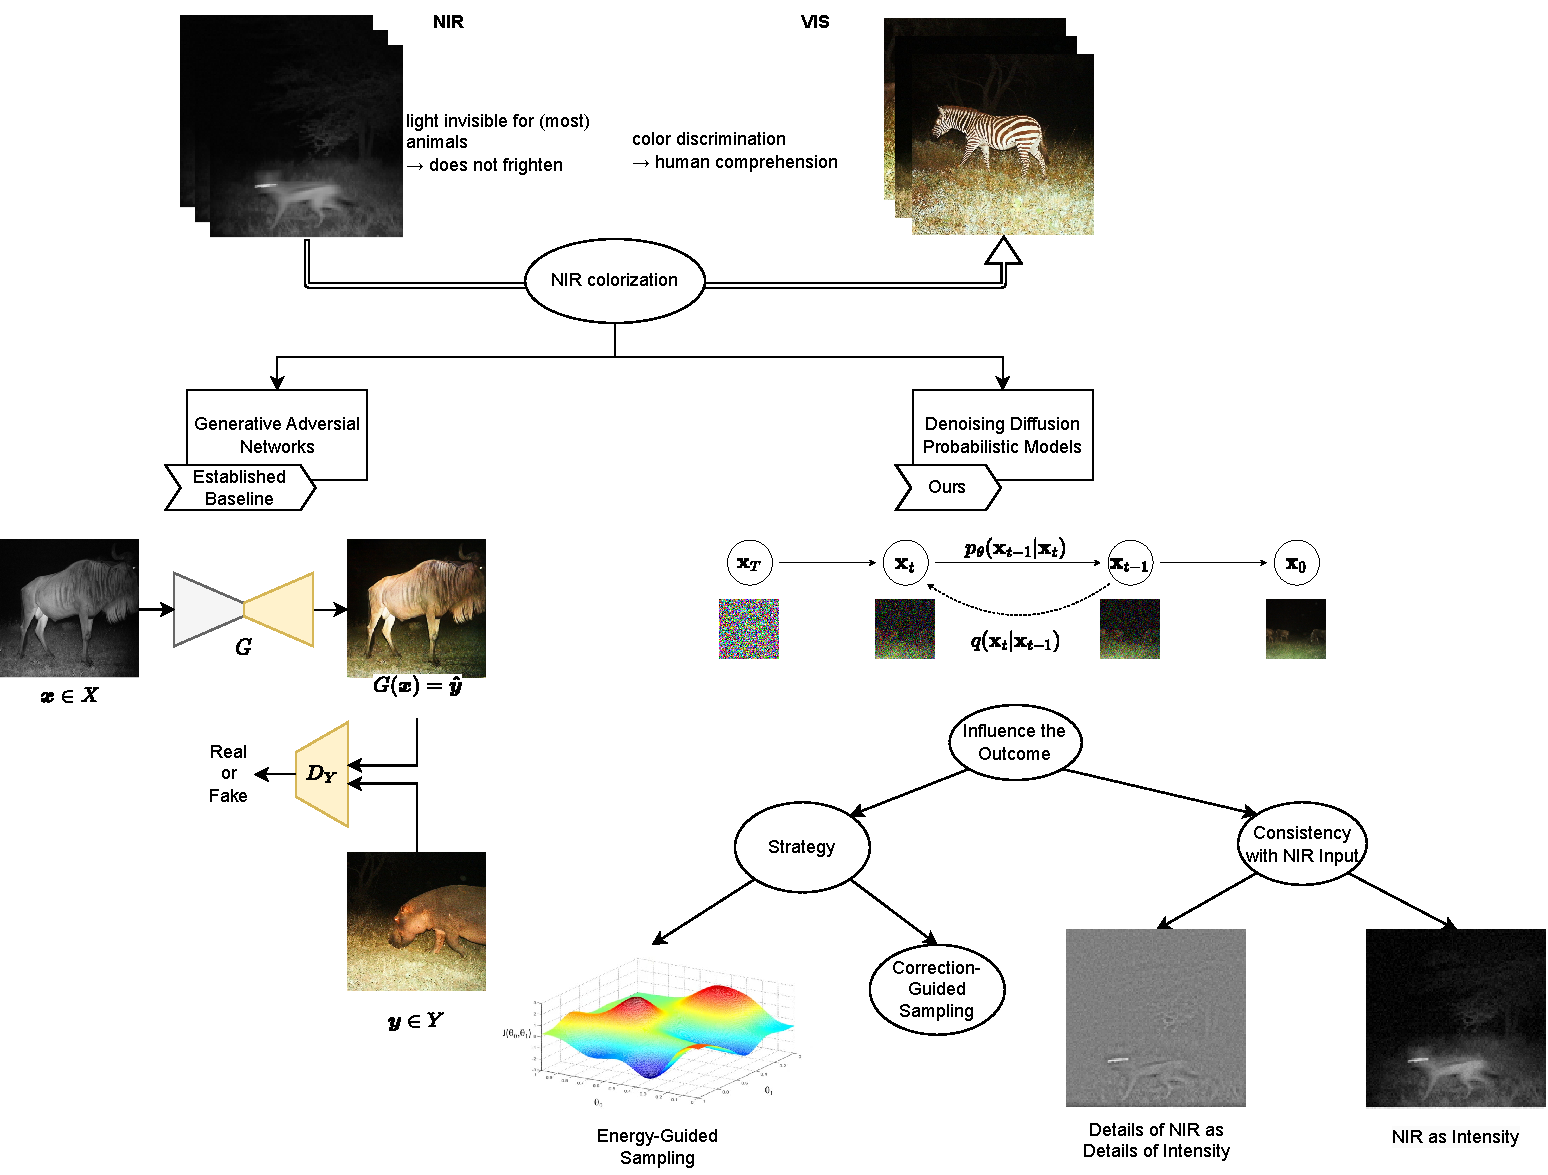
\includegraphics[width=\textwidth]{gfx/Graphical-Abstract.pdf}
    \caption{
        \textbf{Structural overview}.
        Motivated by combining both benefits of near-infrared and visible light images, 
        we develop a novel sampling method based on denoising diffusion probabilistic models \parencite{ddpm} to colorize near-infrared images. 
        We compare our model with current established baselines for NIR colorization: Generative Adversarial Models \parencite{mehri}. 
        While developing our approach we focus on ways to guide the model (\autoref{sec:conditional-sampling}). 
        First we investigate two sampling strategy, the energy-guided (\autoref{sec:energy-guided-sampling}) and correction-guided sampling (\autoref{sec:correction-guided-sampling}). 
        Secondly ways to formulate consistency with the near-infrared image into the sampling process are researched, namely by replacing intensity with the near-infrared images (\autoref{sec:correction-guided-sampling-gray-scale-colorization}) 
        and by replacing only the details of the intensity with those of the near-infrared image (\autoref{sec:correction-guided-sampling-nir-colorization}).
    }
\end{figure}